% 2020 全国Ⅲ卷 理8：某几何体的三视图
% 来源 PDF：普通高考/2020/2020全国3理(云南,广西,贵州,西藏,四川).pdf 第 1 页（A3 横排），印面 1125，第 8 题题干下方
% 结构（按原页矢量数据换算）：主视图、左视图、俯视图均为腰长 2 的等腰直角三角形；
%   主视图直角在右下，左视图直角在左下，俯视图直角在右上。三视图的直角互相对应，
%   故该几何体是三条两两垂直的棱长均为 2 的四面体。
% 尺寸标注：原页只在主视图底边、主视图右边、俯视图右边标出「2」，此处照录。
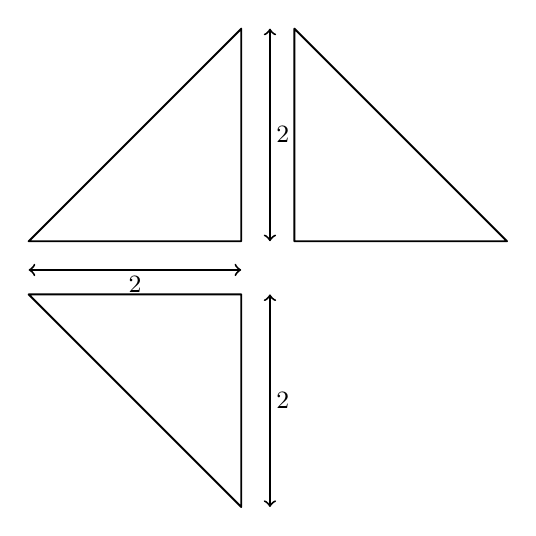
\begin{tikzpicture}[line width=0.7pt, font=\small,
  x=1.35cm, y=1.35cm, line cap=round, line join=round]

  % 主视图：直角边 2 与 2，直角在右下
  \draw (0,0) -- (2,0) -- (2,2) -- cycle;

  % 左视图：直角边 2 与 2，直角在左下
  \draw (2.5,0) -- (4.5,0) -- (2.5,2) -- cycle;

  % 俯视图：直角边 2 与 2，直角在右上
  \draw (0,-0.5) -- (2,-0.5) -- (2,-2.5) -- cycle;

  % 尺寸标注
  \draw[<->] (0,-0.27) -- (2,-0.27) node[midway, below, inner sep=2pt] {$2$};
  \draw[<->] (2.27,0) -- (2.27,2) node[midway, right, inner sep=2pt] {$2$};
  \draw[<->] (2.27,-0.5) -- (2.27,-2.5) node[midway, right, inner sep=2pt] {$2$};
\end{tikzpicture}
